\subsection*{2. プロジェクト管理}

本節では,我々がプロジェクトを円滑に進めるために使用していた管理ツールおよび進捗や問題の報告等を実現するための体制について述べる.
	
今回のプロジェクトへ取り組むにあたり,IoT 機器による BLE 取得や混雑度を可視化するシステムの処理内容を記述したソースコードの管理,
並びにタスクの管理や情報共有を実現するために以下の 3 つのツールを用いた.
	
\begin{enumerate}
	\item \textbf{GitHub}
	
	GitHub とは,Git\cite{Git} を基盤とするリポジトリ(データベース)を用いたソースコード管理と開発者同士のコラボレーションを実現するプラットフォームのことである\cite{GitHub}.
	分散型のソースコード管理では,各開発者がリモートリポジトリとは別にローカルリポジトリを個人のローカルディスクに持ち,
	ローカルリポジトリに対してコミット等の処理を行う仕組みになっているものをいう(図\ref{fig:分散型のバージョン管理}).
	なお,そのままでは開発者間でリポジトリを共通できないため,必要に応じてローカルリポジトリの内容とリモートリポジトリの内容を同期させることになる.
	\begin{figure}[tb]
		\centering
		\includegraphics[scale=0.5]{./fig/distributed\_vcs.pdf}
		\caption{分散型のバージョン管理}
		\label{fig:分散型のバージョン管理}
	\end{figure}
	
	一般に,手元のリポジトリの内容を別のリポジトリへ反映(同期)させることをプッシュ(push)といい,
	逆に別のリポジトリの内容を手元のリポジトリへ取り込む操作のことをプル(pull)という.	
	開発者がローカルリポジトリに対して行ったコミットはそのままではリモートリポジトリに対しては反映されないため,
	変更内容をリモートリポジトリへプッシュする必要がある.
	ただし,誰でも自由にリモートリポジトリへプッシュ操作を行えるわけではなく,通常はそのための権限を持った一部の開発者(管理者)に限られている.
	それゆえ多くの場合,開発者たちは変更内容を管理者へ提示し,それをリモートリポジトリへ反映してもらうよう依頼することになる.
	つまり,管理者がプル操作を行うことで依頼のあったローカルリポジトリの内容をリモートリポジトリへ取り込むことができる.
	そのような依頼のことをプルリクエスト(pull request)といい,分散型バージョン管理システムを使った開発プロジェクトではプルリクエストが 1 つの開発・保守作業単位になっている場合もある.
	
	\item \textbf{Notion}
	
	Notion とは,メモ・タスク管理・ドキュメント作成・データベース機能を統合した多機能な情報管理ツールのことである\cite{Notion}.
	具体的には,Markdown 対応のメモや To-Do リスト・カンバンボードでタスク管理ができるだけでなく,データベース機能により情報を整理・フィルタリングが可能である.
	さらに,リアルタイム共同編集にも対応しており,チームでのプロジェクト管理にも適している.
	これらのようにカスタマイズ性が高いことから,個人から企業まで幅広く活用されている.
	
	我々は,目的を達成するために必要なタスクを洗い出し,Notionの機能を活用して整理を行っていた.
	図\ref{fig:Notionを使ったタスク管理}にその一部の内容を示す.
	\begin{figure}[tb]
		\centering
		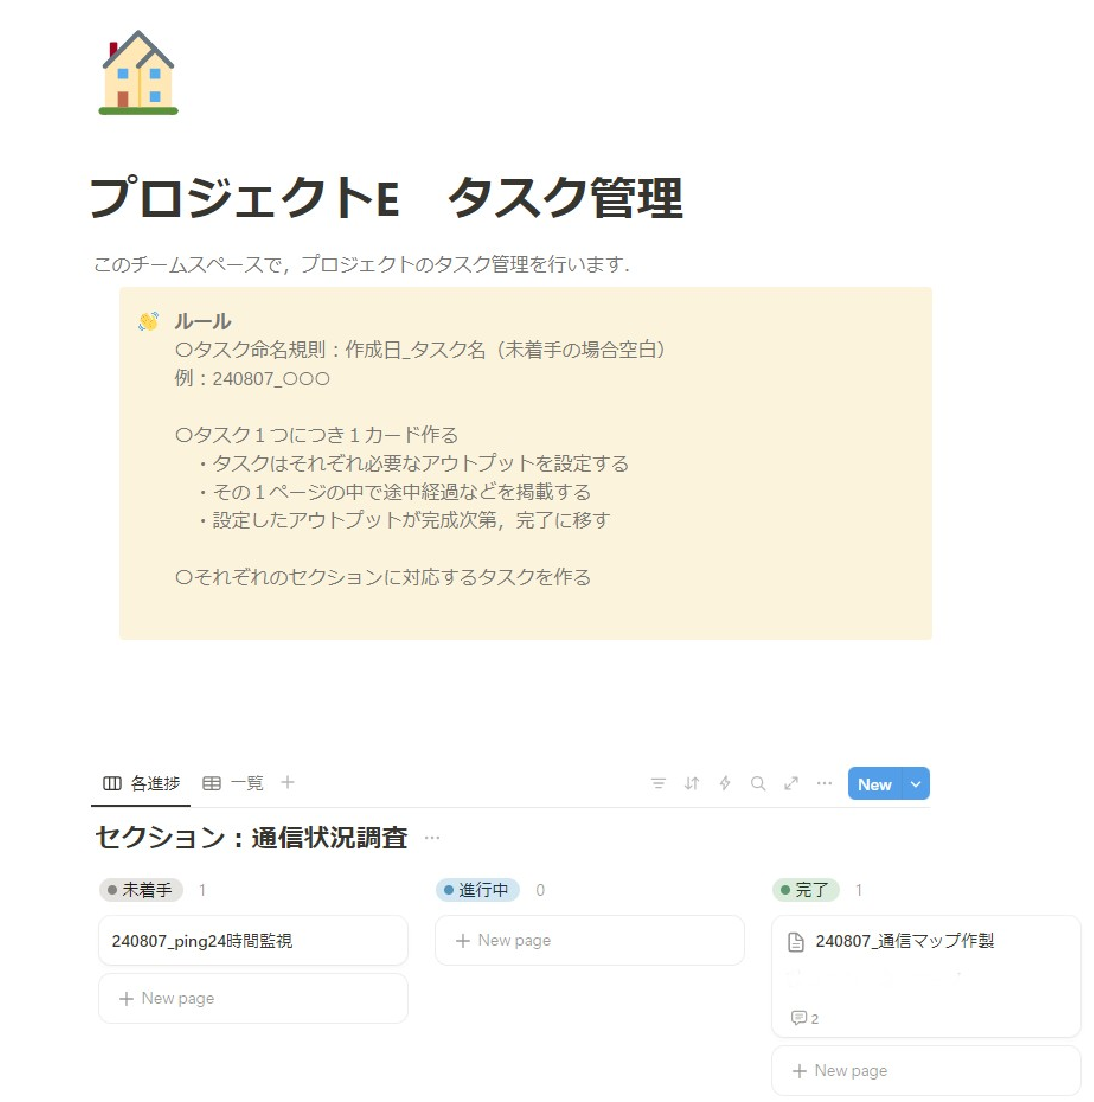
\includegraphics[scale=0.45]{./fig/notion.pdf}
		\caption{Notionを使ったタスク管理}
		\label{fig:Notionを使ったタスク管理}
	\end{figure}
	
	\item \textbf{Discord}
	
	Discord とは,ボイスチャット・テキストチャット・ビデオ通話ができるコミュニケーションツールのことである\cite{Discord}.
	サーバーを作成し,チャンネルごとにメンバーと交流できるためゲーマーやコミュニティ、ビジネス用途にも活用されている.
	
	我々は,連絡手段としてこのツールを活用した.
	例えば,進捗確認や課題の報告を行う週1回の対面定例ミーティングの告知に使用した.
	ミーティングでは、役割ごとにグループ分けされた班が、それぞれ進捗や課題を整理したプレゼン資料を作成し、報告を行った.
\end{enumerate}

